\documentclass{article}


\graphicspath{{../Chapters/2.Vectors/DotProduct/pic/}}
% !TeX root = ../../../Mainfile/book.tex



\begin{document}

\color{white}
\subsection{Vector dot product}
\color{black}

\begin{equation*}
 \icol{\color{rooj} 1 \\ \color{groen} 3 \color{black} } \bullet \icol{\color{rooj} 4 \\ \color{groen} 1 \color{black} } = \color{rooj} 1 \cdot 4  \color{black} + \color{groen}  3 \cdot 1 \color{black} = 7
\end{equation*}





\paragraph{Dot product:} Another useful \textbf{vector operation} is the \textbf{dot product}. Take the product of corresponding elements, and then add together the result. 

\color{theorem} \paragraph{Definition:} \textit{Two vectors $u=\vect{u_1, u_2,\dots,u_n}$ and $v=\vect{v_1,v_2,\dots,v_n}$, of the same dimension (\textbf{n}) have the dot product 
\[
\vec{u}\bullet \vec{v} = u_1\cdot v_1 + u_2\cdot v_2+ \dots u_n\cdot v_n 
\]
or
\[
\vec{u}\bullet \vec{v} = |\vec{u}|\cdot |\vec{v}| \cos \theta_{uv}
\]
where $\theta_{uv}$ is the angle between $\vec{u}$ and $\vec{v}$.
} \color{black}

\paragraph{Uses:} The dot product tells us a lot about the direction of the vectors relative to each other:


\begin{minipage}{0.45\textwidth}
\begin{flushleft}
\textit{Positive dot product}: The angle between the vectors is less than $90^\circ$. 
\end{flushleft}
\end{minipage} \hfill
\begin{minipage}{0.45\textwidth}
\begin{figure}[H]
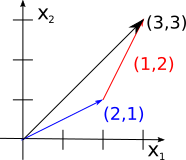
\includegraphics[width = 0.7\linewidth]{1.png}
\end{figure}
\end{minipage}



\begin{minipage}{0.45\textwidth}
\begin{flushleft}
\textit{Dot product is 0}: The vectors are perpendicular to each other, i.e. the angle between them is exactly $90^\circ$. 
\end{flushleft}
\end{minipage} \hfill
\begin{minipage}{0.45\textwidth}
\begin{figure}[H]
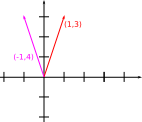
\includegraphics[width = 0.7\linewidth]{2.png}
\end{figure}
\end{minipage}


\begin{minipage}{0.45\textwidth}
\begin{flushleft}
\textit{Negative dot product}: The angle between the vectors is more than $90^\circ$.  
\end{flushleft}
\end{minipage} \hfill
\begin{minipage}{0.45\textwidth}
\begin{figure}[H]
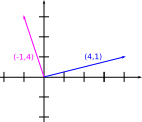
\includegraphics[width = 0.7\linewidth]{3.png}
\end{figure}
\end{minipage}

\

The dot product can even help us find the exact angle between the vectors using the equation in the definition above. If we isolate $\cos \theta_{uv}$ in the equation we get 

\begin{equation} \label{eq:angleDot}
\cos\theta_{uv}=\frac{\vec{u}\bullet\vec{v}}{|\vec{u}|\cdot|\vec{v}|}
\end{equation}

\paragraph{Example:} 

We're gonna find the angle between $\vec{u} = \icol{-4 \\ 2 \\ 8}$

and $\vec{v} = \icol{-3 \\ 5 \\ 1}$.

First we find the dot-product between them

\begin{align*}
\vec{u}\bullet\vec{v} &= (-4\cdot -3)+(2\cdot 5)+(8\cdot 1)\\
&= 12+10+8=30
\end{align*}

We also need their length

\[
|\vec{u}| = \sqrt{(-4)^2+2^2+8^2} = \sqrt{84} 
\]
\[
|\vec{v}| = \sqrt{(-3)^2+5^2+1^2} = \sqrt{35} 
\]

using \eqref{eq:angleDot} we get
\[
\cos \theta_{uv} = \frac{30}{\sqrt{84}\cdot\sqrt{35}}
\]

so the angle is

\[
\theta_{uv} = \cos^{-1} \bigg( \frac{30}{\sqrt{84}\cdot\sqrt{35}}\bigg) \approx 56.4^\circ
\]



\paragraph{Exercise:} Do the same for $\vec{u}=\vect{5,3,-2}$ and $\vec{v}=\vect{2,-2,-1}$.


\end{document}